\documentclass{article}
\usepackage{tikz}

\begin{document}

\centering

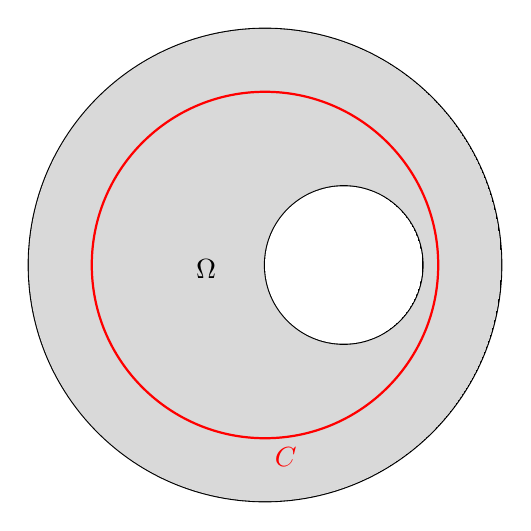
\begin{tikzpicture}[>=stealth]
    % Teken de buitencontour en maak grijs
    \draw[thick] (0,0) circle(3);
    \begin{scope}
        \clip (0,0) circle(3); % Knip gebied binnen de buitencontour
        \fill[gray!30] (0,0) circle(3); % Kleur het gebied tussen de cirkels
    \end{scope}
    
    % Teken de binnencontour (kleinere cirkel)
    \draw[thick] (1,0) circle(1);
    \begin{scope}
        \clip (1,0) circle(1); % Knip gebied binnen de buitencontour
        \fill[white] (1,0) circle(1); % Kleur het gebied tussen de cirkels
    \end{scope}

    % Teken C2 (gesloten contour rond de binnencontour)
    \draw[thick,red] (0,0) circle(2.2);
    \node[below right,red] at (0,-2.2) {$C$};
    \node[above right] at (-1,-0.3) {$\Omega$};
\end{tikzpicture}
\end{document}